\section{Results and comparison}
%
% REMARK. testcases are run for about 900 seconds. iter/sec was taken from the last entry
%         started with ./nltool -i ../hash/sha2/chars/sha256/startchars/27-t10.xml
%
%\begin{table}[t]
\begin{sidewaystable}
 \begin{center}
  \begin{tabular}{lccccc}
                               & \multicolumn{3}{c}{1 additional bit condition requires in average} & \\
   Approach                    & boolean vars & clauses & assumptions   & performance \\
  \hline
   Simple evaluation           & $2.0$        & $1.375$ & $0$           & $\approx117$ iter/sec \\  % TODO: verify: does it really always recreate the SAT solver
   % lp/sat: Info: seed 2236221566 time: 893 iter/sec: 122 iterations: 4081 stak_soze: 95 contr: 463 restarts: 329 minfree: 0 absminfree: 0 credits: 9537 phase: 1 found :0 smax: 95 complete: 1/1 0/0
   Activation literals         & $7.0$        & $6$     & $5.6875$      & N/A \\
   Exhaustive encoding         & $17$         & $46$    & $1$           & N/A \\
   Reduced encoding            & $9$          & $20$    & $1.25$        & $\approx177$ iter/sec \\
   % RE: Info: seed 1645337080 time: 894 iter/sec: 177 iterations: 123 stack_size: 0 contr: 3 restarts: 459 minfree: 152 absminfree: 0 credits: 9997 phase: 0 found: 0 smax: 2 complete: 0/0
   Differential state encoding & $4$          & $7$     & $1.5$         & ? \\
   % DSE: Info: seed 1967938805 time: 567 iterations/sec: 8 iterations: 332 stack_size: 4 contr: 19 restarts: 15 minfree: 116 absminfree: 79 credits: 9981 phase: 0 found: 0 smax: 7 complete: 0/0
  \end{tabular}
  \caption[All encodings in comparison]{
    All encodings in comparison.
    The number of variables and clauses is not important in the first place, but will influence the SAT solvers performance.
    A small number of assumptions is desirable in any case.
  }
  \label{tab:encoding-cmp}
 \end{center}
%\end{table}
\end{sidewaystable}

Simple evaluation obviously has the worst performance. Destroying and building the SAT solver takes a lot of time and slows down the automated search. The advantage of this approach comes into play, when the evaluated differential characteristic is very large. However this size is not within the scope for SAT-based attacks of hash algorithms.

The approaches for Activation literals, Reduced encoding and Differential state encoding all seem interesting and perform very good. Further study is advised to improve the speed by studying the recurring structures due to assigned bit conditions.

\section{Propagation}
%
The propagation in the automated search improved previous implementation, because overlapping bits are detected and considered. Therefore the implementation scales better for larger sizes, because invalid paths are eliminated faster. Figure~\ref{fig:sat-propagation} can directly be compared to the propagation diagrams given in~\cite{Cry16}.
%
\begin{figure}[t]
 \begin{center}
  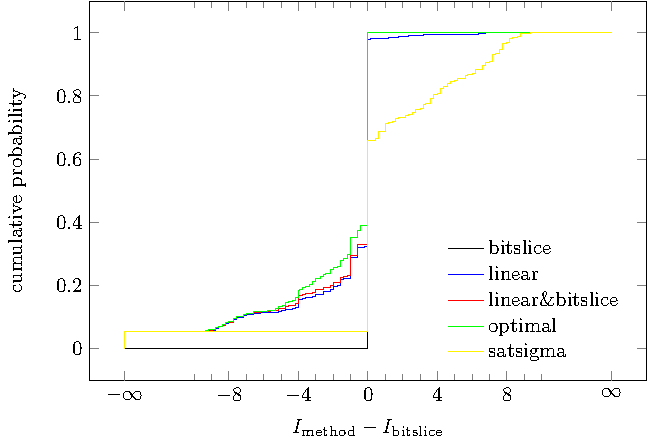
\includegraphics{img/propagation.pdf}
  \caption[Comparison of propagation methods.]{Comparison of propagation methods. Higher values means better propagation.}
  \label{fig:sat-propagation}
 \end{center}
\end{figure}

\section{Implementation-dependent improvements}
%
\begin{itemize}
  \item Tests shall be made also with different state-of-the-art SAT solvers from different families of the DPLL algorithm such that comparison is possible.
  \item An implementation of the activation literal approach is desirable.
  \item The truth table is a bottleneck of the Initialization step. Tests are required whether approaches like Tseitin's Definitional Normal Form perform better as discussed in~\cite{Sat03}.
  \item SAT solvers themselves propagate values in their evaluation. The same concept is desirable in \nltool. Strategies to put SAT solver technology directly into the framework shall be discussed.
  \item Any fast simplification algorithms for boolean equations are of interest. In the initialization step all clauses are already known. Performing a simplification algorithm especially to the clauses of the primitive functions might lead to a speedup. Karnaugh maps, the Quine-McCluskey algorithm and the Espresso algorithm shall be considered. Simplification algorithms have been implemented by Akawat Homsirikamol et~al.~\cite{Cry04} with HDL in the Quartus II software.
\end{itemize}

\section{Independent approaches}
%
\begin{itemize}
  \item SMT solvers and STP allow a more powerful encoding of the problem to solve. This deprecates the usage of truth tables and encodings. A comparison is of interest.
\end{itemize}
